\documentclass[xcolor=table]{beamer}
\usetheme{Warsaw}

%\useoutertheme{infolines}
%\useinnertheme{circles}
\usepackage[utf8]{inputenc}
\usepackage{amsmath}
\usepackage{amsfonts}
\usepackage{amssymb}
% \usepackage{graphicx}
\usepackage{graphicx,epsfig}

\usepackage{textpos} 
\usepackage{listings}
\usepackage{hyperref}
\usepackage{multirow}
\usepackage{multicol}

\newcommand{\logoSENAC}{images/etec-small.png}
\newcommand{\logoUFSCar}{images/LogoUfscar.eps}
%\logo{\includegraphics[width=0.18\textwidth]{images/logoFATEC.png}\vspace{220pt}}


\setbeamertemplate{headline}{%
%\leavevmode%
%  \hbox{%
%    \begin{beamercolorbox}[wd=\paperwidth,ht=2.5ex,dp=1.125ex]{palette quaternary}%
%    \insertsectionnavigationhorizontal{\paperwidth}{}{\hskip0pt plus1filll}
%    \end{beamercolorbox}%
%  }

}

\addtobeamertemplate{frametitle}{}{%
	
	\small{
	
    \begin{textblock*}{\textwidth}(0cm,0.1cm)
		%\insertsectionnavigationhorizontal{\paperwidth}{}{\hskip0pt plus1filll}
%		\textcolor{gray}{\insertsectionhead\insertsubsectionhead}
		 
		
		%\insertsection \insertsubsection
    \end{textblock*}
	}
    




	% \begin{textblock*}{100mm}(0.93\textwidth,-0.55cm)
        % \includegraphics[width=0.15\textwidth]{\logoUFSCar}
    % \end{textblock*}




%    \begin{textblock*}{100mm}(0.93\textwidth,-0.75cm)
%        \includegraphics[width=0.1\textwidth]{\logoSENAC}
%    \end{textblock*}
}


\institute[]{
  %\inst{1}
  \includegraphics[width=0.25\textwidth]{\logoUFSCar}
} 

\setbeamercovered{transparent} 
\setbeamertemplate{navigation symbols}{} 
\setbeamercovered{invisible}




% \setbeamertemplate{footline}{% 
  % \hfill% 
  % \usebeamercolor[fg]{page number in head/foot}% 
  % \usebeamerfont{page number in head/foot}% 
  % \insertframenumber%
  % %\,/\,\inserttotalframenumber
  % \kern1em\vskip2pt% 
% }




% https://tex.stackexchange.com/questions/333587/beamer-frame-number-without-total/333684
\setbeamertemplate{footline}{
  \hfill%
  \usebeamercolor[fg]{page number in head/foot}%
  \usebeamerfont{page number in head/foot}%
  \insertframenumber%
  % \setbeamertemplate{page number in head/foot}[framenumber]%
  \usebeamertemplate*{page number in head/foot}\kern1em\vskip5pt%
}



%gets rid of bottom navigation bars
% \setbeamertemplate{footline}[frame number]{}
% \setbeamertemplate{footline}{\insertframenumber }



% \setbeamertemplate {footline}{\quad\hfill\insertframenumber\strut\quad}




% \setbeamertemplate{sidebar right}{}
% \setbeamertemplate{footline}{%
% \hfill\usebeamertemplate***{navigation symbols}
% \hspace{1cm}\insertframenumber{}}



% Define o caminho das figuras
\graphicspath{{images/}}

%\AtBeginSection[] 
%{
%    \begin{frame}
%	    \frametitle{Roteiro}
%	    \tableofcontents[currentsection]
%    \end{frame}
%}


%https://bloerg.net/2012/06/21/customizing-the-frametitle-of-beamer-presentation.html




\AtBeginSection[] 
{
    \begin{frame}
	    \frametitle{Roteiro}
	    \tableofcontents[currentsection]
    \end{frame}
}












%%%%%%%%%%%%%%%%%%%%%%%%%%%%%%%%%%%%%%%%%%%%%%%%%%%%%%%%%%%%%%%%%%%%%%%%%%%%%%%%%%%%
%%%%%%%%%%%%%%%%%%%%%%%%%%%%%%%%%%%%%%%%%%%%%%%%%%%%%%%%%%%%%%%%%%%%%%%%%%%%%%%%%%%%

\newcommand{\sumario}{
\begin{frame}[plain]
   \frametitle{Plano de Aula}
   \tableofcontents
\end{frame}
}

\newcommand{\frameTalkIsCheap}{
\begin{frame}{Exercícios}

	\addimage{images/talkischeap3}{0.65}{}

	\begin{flushright}
		Linus Torvalds
	\end{flushright}
\end{frame}		
}

\newcommand{\frameDuvidas}{
\begin{frame}{Dúvidas?}
	\addimage{images/questions.png}{0.65}{}
	 	
\end{frame}		
}


\newcommand{\addimage}[2]{
  \begin{figure}[!h]
  \centering
  \includegraphics[width=#2\paperwidth]{#1}
%  \caption{#3}
%  \label{fig:#4}
  \end{figure}
}


\newcommand{\addpdfpageh}[4]{
\includegraphics[trim={#1cm #2cm #1cm #2cm},clip,page=#4,height=0.8\paperheight]{#3}
}
\newcommand{\addpdfpagew}[4]{
\includegraphics[trim={#1cm #2cm #1cm #2cm},clip,page=#4,width=0.8\paperwidth]{#3}
}


%%%%%%%%%%%%%%%%%%%%%%%%%%
% blocks
%%%%%%%%%%%%%%%%%%%%%%%%%%

\newcommand{\popc}[2]{
\begin{block}{#1}
	\pause	
	#2
\end{block}
}

\newcommand{\pop}[2]{
\pause	
\begin{block}{#1}
	#2
\end{block}
}

\newcommand{\nblock}[2]{
\begin{block}{#1}
	#2
\end{block}
}

\newcommand{\eblock}[2]{
\begin{exampleblock}{#1}
	#2
\end{exampleblock}
}

\newcommand{\ablock}[2]{
\begin{alertblock}{#1}
	#2
\end{alertblock}
}



% Uma macro que cria \newenvironments
\newcommand{\coloredblock}[3]{
	\newenvironment{#1}[1]
	{
		\setbeamercolor{block title}{fg=white,bg=#2!75!black}%
		\begin{block}{#3}
	}
	{
		\end{block}
	}	
}

% Criaçao de \newenvironments
\coloredblock{blackblockenv}{black}{#1}
\coloredblock{blueblockenv}{blue}{#1}
\coloredblock{redblockenv}{red}{#1}

% Macro para chamar as \newenvironments criadas
\newcommand{\blackblock}[2]{
	\begin{blackblockenv}{#1}
		#2
	\end{blackblockenv}
}
\newcommand{\redblock}[2]{
	\begin{redblockenv}{#1}
		#2
	\end{redblockenv}
}
\newcommand{\blueblock}[2]{
	\begin{blueblockenv}{#1}
		#2
	\end{blueblockenv}
}









%\newcommand{\coloredblock}[3]{
%	\setbeamercolor{block title}{fg=white,bg=#1!75!black}%
%	\begin{block}{#2}
%		#3
%	\end{block}
%}
%
%\newcommand{\redblock}[2]{
%	\coloredblock{red}{#1}{#2}
%}
%
%\newcommand{\yblock}[2]{
%	\setbeamercolor{block title}{fg=white,bg=yellow!75!black}%
%	\begin{block}{#1}
%		#2
%	\end{block}
%}



%\newenvironment<>{myblock}[1]
%{%
%	\setbeamercolor{block title}{fg=white,bg=red!75!black}%
%	\begin{block}#2{#1}
%}
%{
%	\end{block}
%}
%  
%
%
%\newenvironment{blueblock}[1]
%{
%	\setbeamercolor{block title}{fg=white,bg=blue!75!black}%
%	\begin{block}{#1}
%}
%{
%	\end{block}
%}
%
%
%
%
%\newcommand{\mblock}[2]{
%\begin{block}{#1}
%	#2
%\end{block}
%}

%
%
%% Uma macro que cria \newenvironments
%\newcommand{\coloredblock}[3]{
%
%	\newenvironment{#1}[1]
%	{
%		\setbeamercolor{block title}{fg=white,bg=#2!75!black}%
%		\begin{block}{#3}
%	}
%	{
%		\end{block}
%	}
%	
%}
%
%% Criaçao de \newenvironment 
%\coloredblock{preto}{black}{#1}
%
%% Macro para chamar as \newenvironment criadas
%\newcommand{\blackblock}[2]{
%	\begin{preto}{#1}
%		#2
%	\end{preto}
%}

\author{Ovídio José Francisco\\
Orientadora: Prof.ª Dr. Katti Faceli\\
Coorientador: Prof. Dr. Rafael Geraldeli Rossi}
\title{Avaliação de Técnicas de Recuperação de Informação
para Organização e Extração de Conhecimento de Documentos de Reunião} 
\subtitle{}
% \date{\today} 
\subject{Dissertação de Mestrado} 


\begin{document}

\begin{frame}
	\titlepage
	 \begin{center}{}\end{center} 
\end{frame}
%\sumario

   \begin{frame}
		\frametitle{Roteiro}
		\tableofcontents
   \end{frame}

%\section{Introdução}
\section{Contextualização}



\begin{frame}{Contexto}

As atas registram assuntos discutidos em reuniões e podem ser utilizadas como base de dados.
\nblock{}{
\begin{itemize}
	\item Utilizadas como referência e apoio a decisões; 
	\item Um assunto pode ser discutido diversas vezes em reuniões diferentes;
	\item É desejável recuperar um histórico desses assuntos ao longo do tempo;
	\item Necessidade de ferramentas automáticas.
\end{itemize}
}

\end{frame}




\begin{frame}{Contexto}

Recuperação de Informação em documentos textuais:

\nblock{}{
\begin{itemize}
	\item Informações contidas em grandes quantidades de texto;
	\item Inerentemente não estruturados;
	\item Documentos com múltiplos assuntos;
	\item Assuntos dispersos pela base de documentos.
\end{itemize}
}

\end{frame}



\begin{frame}{Contexto}

% Um dos principais desafios nesse cenário é 
Nesse cenário, o desafio é encontrar trechos de texto que tratem somente do assunto pesquisado.

\nblock{}{

Essa tarefa consiste em 2 passos principais:
% Essa tarefa tem 2 passos principais:

\begin{itemize}
	\item Encontrar pontos onde há transição de assuntos;
	\item Identificar o teor desses assuntos;
\end{itemize}

} 

\end{frame}





\begin{frame}{Contexto}

% Os algoritmos de segmentação textual são utilizados para dividir um texto em segmentos contendo um assunto completo e relativamente independente.

% \addimage{images/pre-process.png}{.9}{}

\nblock{}{
Algoritmos de Segmentação Textual:

\begin{itemize}
	\item Divide um texto em trechos com um único assunto completo;
	\item Úteis em aplicações com textos sem indicações de quebras de assunto, como transcrições de áudio, e diálogos em chats;
	\item Podem ser uma etapa de pré-processamento para outras aplicações;
	\item Não dão indicações sobre o conteúdo dos segmentos.
\end{itemize}
} 


% \addimage{images/pre-process.png}{.8}{}


\end{frame}





\begin{frame}{Contexto}

% \nblock{}{
	% As técnicas de Extração de Tópicos são empregadas na organização de documentos.
	% Os modelos de Extração de Tópicos podem estimar o assunto de cada documento de uma coleção.
% } 

\nblock{}{
Modelos de Extração de Tópicos:
\begin{itemize}
	\item Estimam o assunto de cada documento de uma coleção;
	\item Agrupam documentos por tópico;
	\item Identificam palavras para descrever os tópicos;
	\item Incorporam conhecimento de domínio aos dados.
\end{itemize}
} 

\end{frame}




\begin{frame}{Trabalhos Relacionados}

		\begin{itemize}
			\item Web document clustering (1998); 
			\item Multi-topic multi-document summarization  (2000); 
			\item Multi-document topic segmentation (2010); 
			\item A Study on Statistical Generation of a Hierarchical Structure of Topic-information for Multi-documents (2011); 
			\item A segment-based approach to clustering multi-topic documents (2013).

		\end{itemize} 

\end{frame}






% ---------- Objetivos ----------
\section{Objetivos}
\begin{frame}{Objetivos}


\nblock{}{
	Propor uma solução para identificar, organizar e consultar assuntos registrados em atas de reunião.  
} 

\nblock{}{
	Utilizar técnicas de Segmentação textual em conjunto com modelos de Extração de Tópicos para:
	\begin{itemize}
	\item Gerar uma estrutura mais organizada que a coleção original.
	\item Utilizar a estrutura latente dos segmentos para Recuperação de Informação. 
	\end{itemize}
}
	% \item Dar início a investigação dessa abordagem no contexto de atas de reunião.


\end{frame}


% ---------- Proposta ----------
\section{Proposta}



\begin{frame}{Visão Geral do Sistema}

	\addimage{images/visao-geral-3.eps}{.8}{}

\end{frame}





\begin{frame}{Módulo de Preparação}
	
	\nblock{Preparação}{
		\begin{itemize}
			\item Extração de texto plano;
			\item Segmentação;
			\item Remoção de termos;
			\item Representação dos Segmentos.
		\end{itemize}
	}
	
	\nblock{Extração de Conhecimento}{
		\begin{itemize}
			\item Extração de tópicos;
			\item Classificação;
		\end{itemize}
	}

	\nblock{Manutenção}{
		Realimentação do sistema	
	}


\end{frame}



\begin{frame}{Preparação}

	\addimage{images/pre-process.png}{.9}{}

\end{frame}




\begin{frame}{Extração de Conhecimento}

	\begin{figure}[h!]

		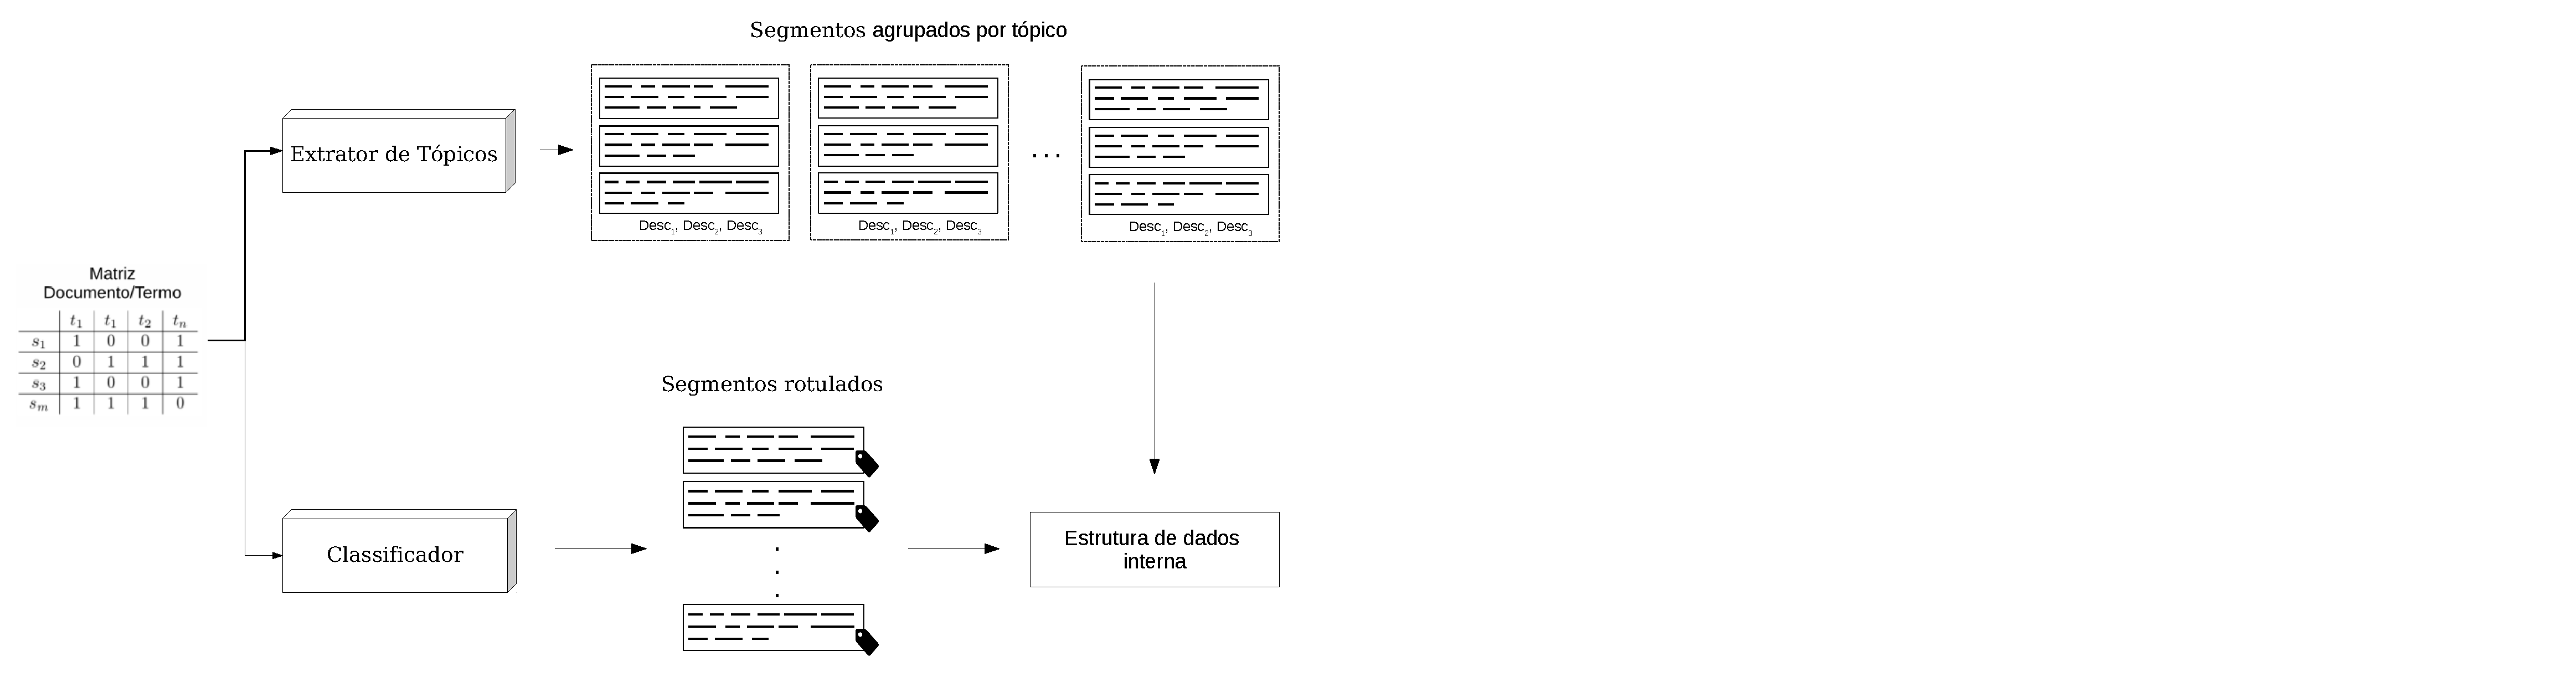
\includegraphics[trim={ 0 2 0 16 },clip,page=1,width=2\textwidth]{images/extracao-conhecimento3.pdf}

	\end{figure}

\end{frame}


\begin{frame}{Estrutura de dados interna}

	% \center Estrutura de dados interna e seu processo de geração.

	\addimage{images/estrutura.png}{.8}{}

\end{frame}

\begin{frame}{Estrutura de dados interna}
	\nblock{}{
		Obtém-se uma estrutura:
		\begin{itemize}
			\item Mais organizada que a coleção original;
			\item Assuntos concentrados em grupos;
			\item Acrescida de novos atributos;
			\item Distribuição dos tópicos conhecida.
			
		\end{itemize}
	}
\end{frame}












\begin{frame}{Distribuição de tópicos em uma ata real}

	\begin{figure}[h!]

		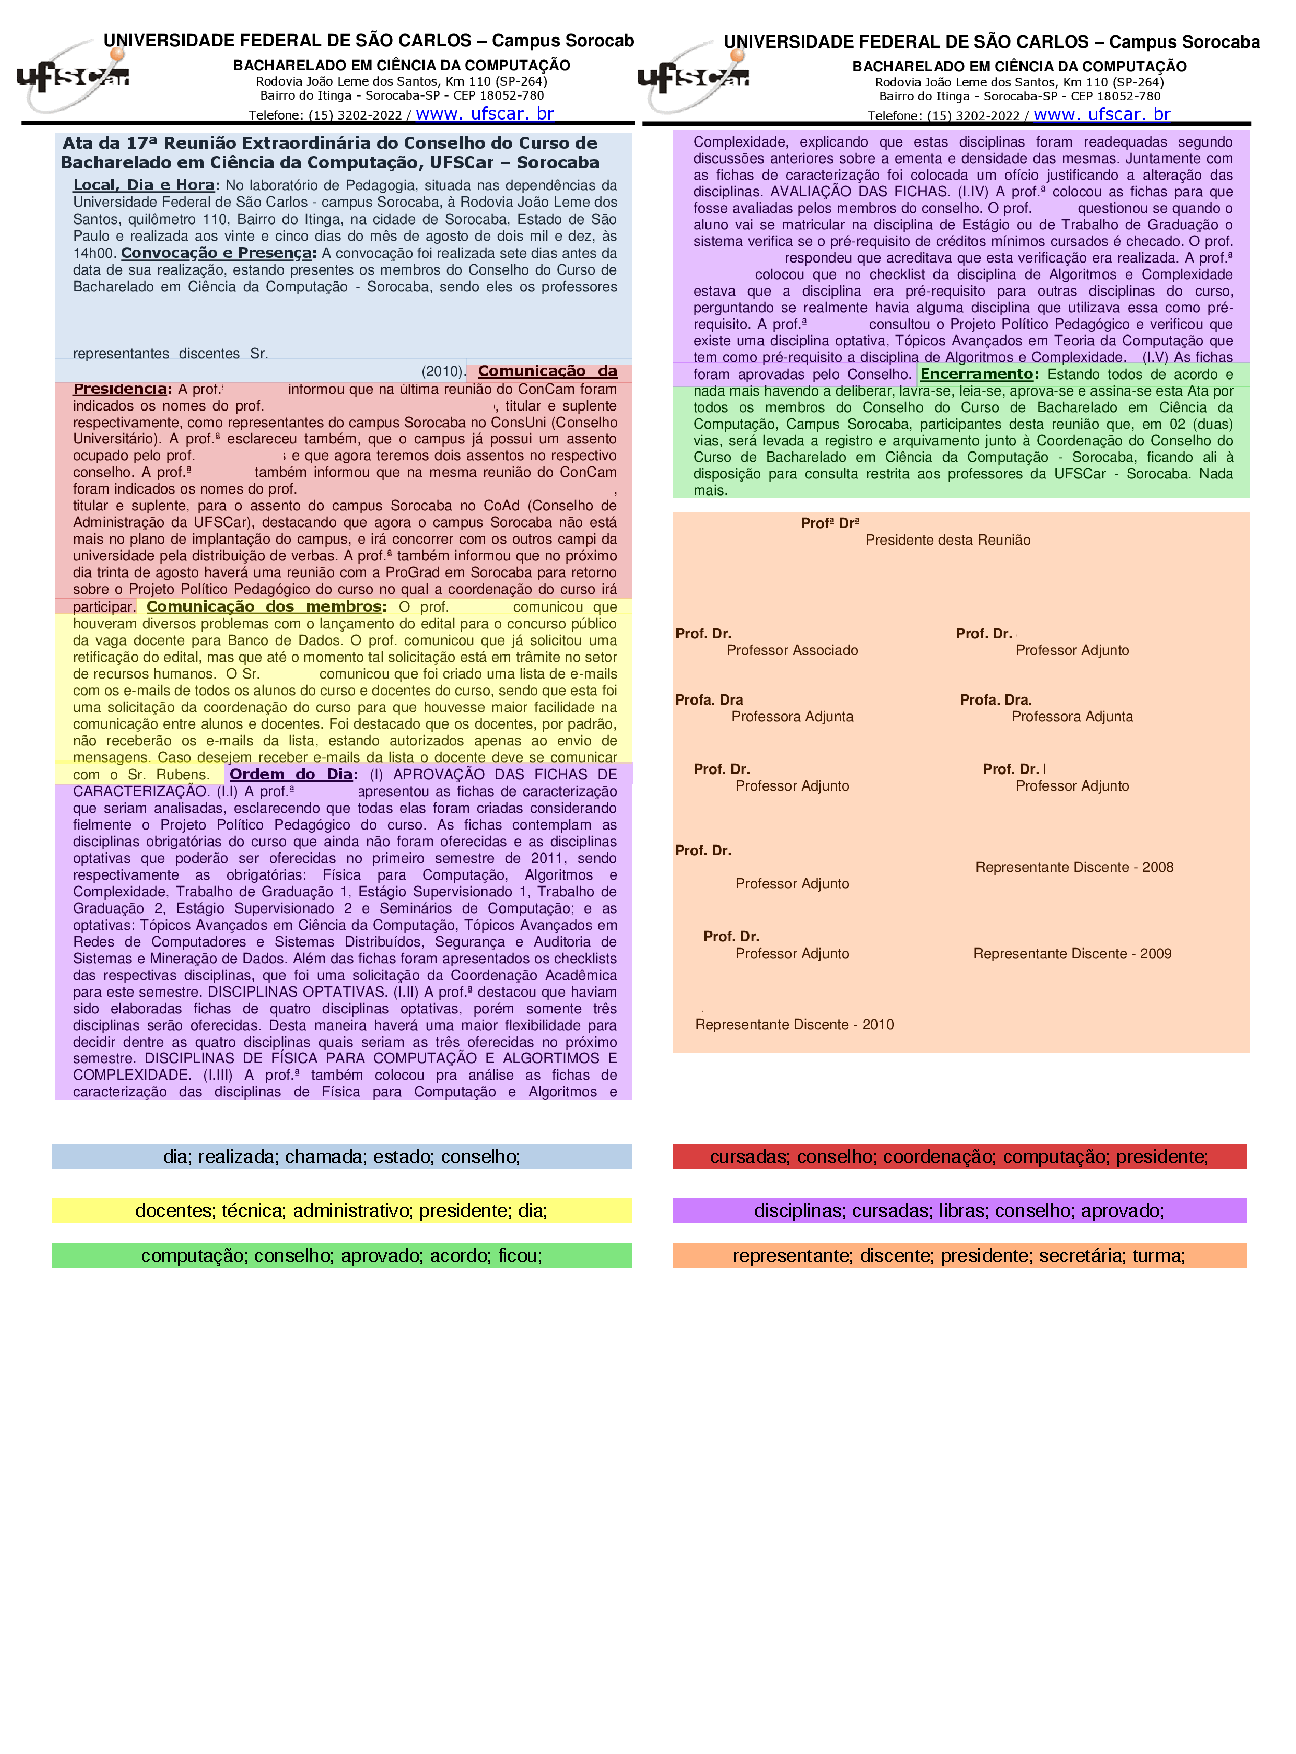
\includegraphics[trim={ 0 265 0 16 },clip,page=1,width=0.85\textwidth]{images/distribuicao.pdf}

	\end{figure}

\end{frame}








\begin{frame}{Distribuição de tópicos em uma ata real} 
	\begin{figure}[h!]

		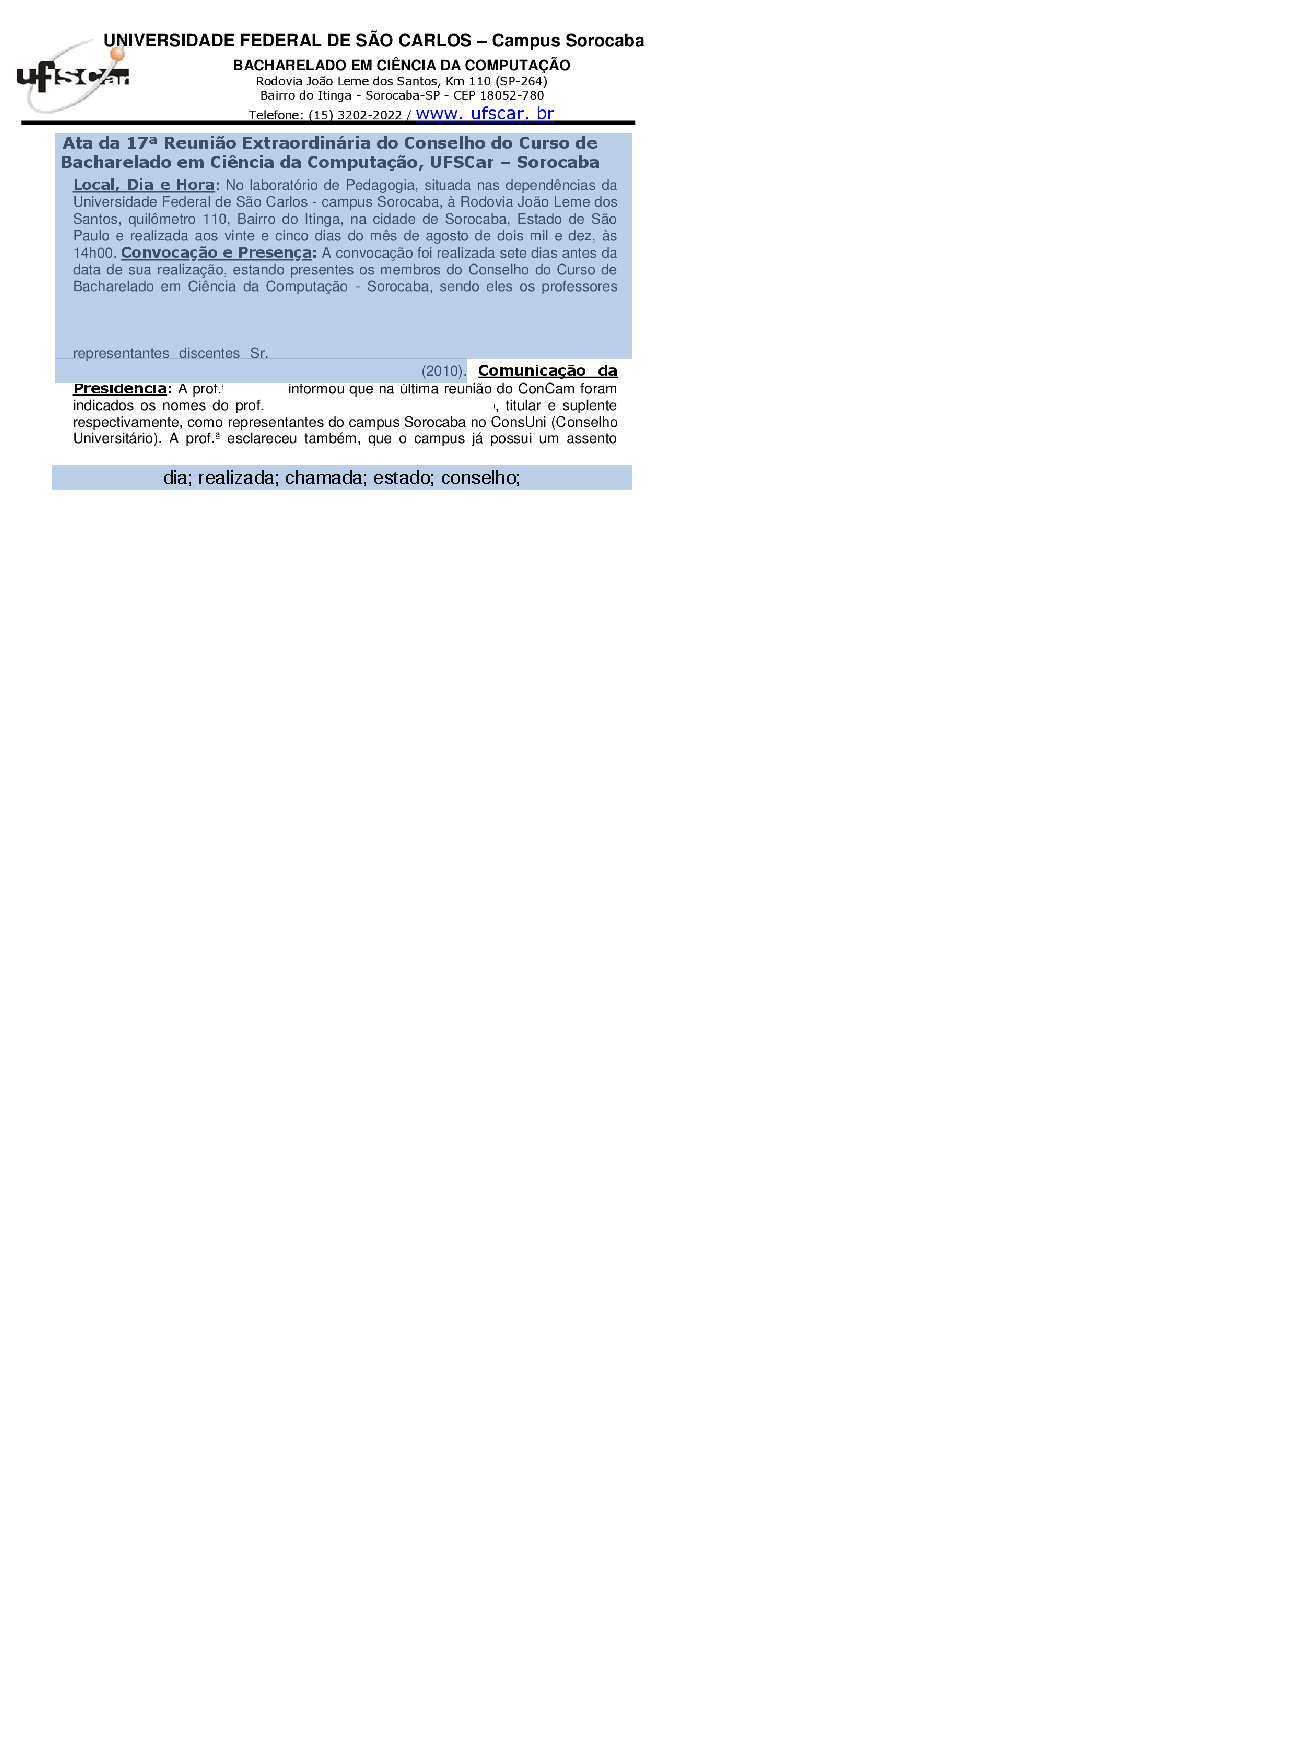
\includegraphics[trim={ 0 565 300 16 },clip,page=1,width=0.95\textwidth]{images/distribuicao-3-parts.pdf}

	\end{figure} 
\end{frame}


\begin{frame}{Distribuição de tópicos em uma ata real} 
	\begin{figure}[h!]

		\includegraphics[trim={ 0 495 300 126 },clip,page=2,width=0.95\textwidth]{images/distribuicao-3-parts.pdf}

	\end{figure} 
\end{frame}


\begin{frame}{Distribuição de tópicos em uma ata real} 
	\begin{figure}[h!]

		\includegraphics[trim={ 0 405 300 256 },clip,page=3,width=0.95\textwidth]{images/distribuicao-3-parts.pdf}

	\end{figure} 
\end{frame}


\begin{frame}{Distribuição de tópicos em uma ata real} 
	\begin{figure}[h!]

		\includegraphics[trim={ 0 320 300 110 },clip,page=4,width=0.60\textwidth]{images/distribuicao-3-parts.pdf}

	\end{figure} 
\end{frame}



\begin{frame}{Distribuição de tópicos em uma ata real} 
	\begin{figure}[h!]

		\includegraphics[trim={ 0 505 300 135 },clip,page=5,width=0.95\textwidth]{images/distribuicao-3-parts.pdf}

	\end{figure} 
\end{frame}


\begin{frame}{Distribuição de tópicos em uma ata real} 
	\begin{figure}[h!]

		\includegraphics[trim={ 0 305 300 195 },clip,page=6,width=0.75\textwidth]{images/distribuicao-3-parts.pdf}

	\end{figure} 
\end{frame}









\begin{frame}{Módulo de Consulta}

	\nblock{ } {
		Módulo de Consulta:
		\begin{itemize}
			\item Utiliza a Estrutura de Dados Interna;
			\item Os tópicos são representados por seus descritores;
			\item Usa-se o Modelo de Espaço Vetorial para ranquear os tópicos;
			\item Exibe-se os segmentos atribuídos ao primeiro tópico do ranking;
			% \item Busca exploratória pelos tópicos mais similares à consulta.
		\end{itemize}
	}

% como os dados são apresentados?
% - Tópico com maior similaridade com a consulta
	% - MSV 

	% (expansão de espaço?)

% \nblock{ } {
	% \begin{itemize}
		% \item O Módulo de Consulta recebe consultas do usuário.
		% \item A Estrutura de Dados Interna é aproveitada para Recuperação de Informação.
	% \end{itemize}
% }

% A Estrutura de Dados Interna é aproveitada para Recuperação de Informação.


% \nblock{ Estrutura mais organizada} {
	% \begin{itemize}
		% \item  Segmentos agrupados por tópico.
		% \item  Segmentos acrescidos de novos atributos (descritores)
	% \end{itemize}
% }


\end{frame}


\begin{frame}{Módulo de Consulta}

	\center Interface do Sistema após uma consulta\\
	\vspace{.5cm}
		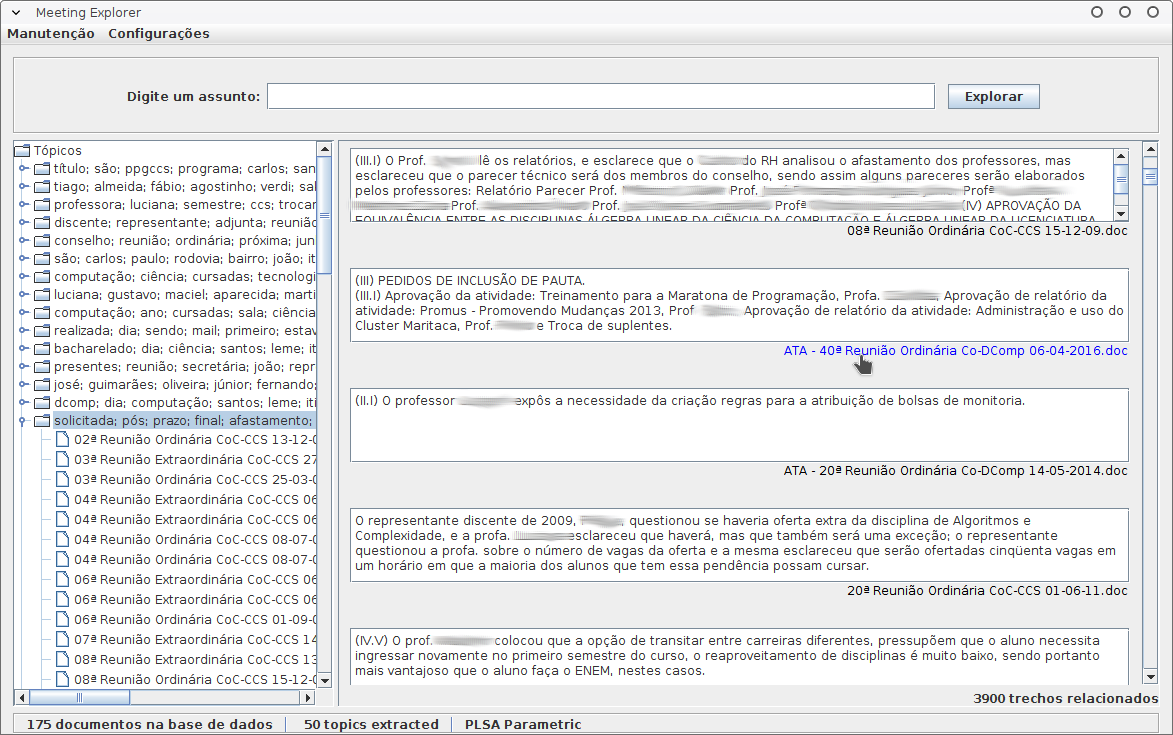
\includegraphics[width=\textwidth]{images/tela-principal-2-1.png}


\end{frame}




\begin{frame}{Sistema}


	\nblock{}{
	 
		O sistema permite:\\
		\begin{itemize}
			\item Receber uma base de dados não estruturada;
			\item Identificar os assuntos tratados em cada ata; 
			\item Agrupar segmentos por tópico;
			\item Adicionar novos atributos (descritores) aos segmentos;
			% \item Incorporar conhecimento de domínio aos dados.
			\item Expandir o espaço de busca; 
			\item Retornar trechos relevantes à consulta.
		\end{itemize}
}
\end{frame}
 



 





% ---------- Análise dos Resultados ----------
 
 
\section{Avaliação Experimental}
\begin{frame}{Avaliação Experimental}

	Os segmentadores foram avaliados objetivamente. 
	\nblock{}{
\begin{itemize}
	\item Processo de anotação manual em segmentos;		
	\item Criação de segmentações de referência;
	\item Configuração dos algoritmos;
	\item Medidas de desempenho (Acurácia, F$^1$, WindowDiff e P$_k$).
	 % entre a referência e os segmentos obtidos.
\end{itemize}
}


\eblock{}{
\begin{itemize}
	\item \textit{Testes de significância estatística (Friedman e Nemenyi)}
\end{itemize}
}

\end{frame}





\begin{frame}{Processo de anotação manual em segmentos}


	\nblock{}{
		A tarefa dos anotadores consistiu em:
		\begin{itemize}
			\item Selecionar trechos com um único assunto;
			\item Rotular os trechos selecionados;
				\begin{itemize}
					\item Tipo comunicação;
					\item Contexto onde se gerou o assunto;
					\item Descrição do assunto.
				\end{itemize} 
			% \item 
		\end{itemize} 
	}

	\nblock{}{
		Utilizou-se:
		\begin{itemize}
			\item 12 atas da UFSCar;
				% \begin{itemize}
					% \item 6 do 
				% \end{itemize} 
			\item 09 anotadores;
			\item Ferramenta para anotações em segmentos.
		\end{itemize} 

	}
\end{frame}







\begin{frame}{Processo de anotação manual em segmentos}
	\center Ferramenta desenvolvida para anotação em segmentos\\
	\vspace{.5cm}
		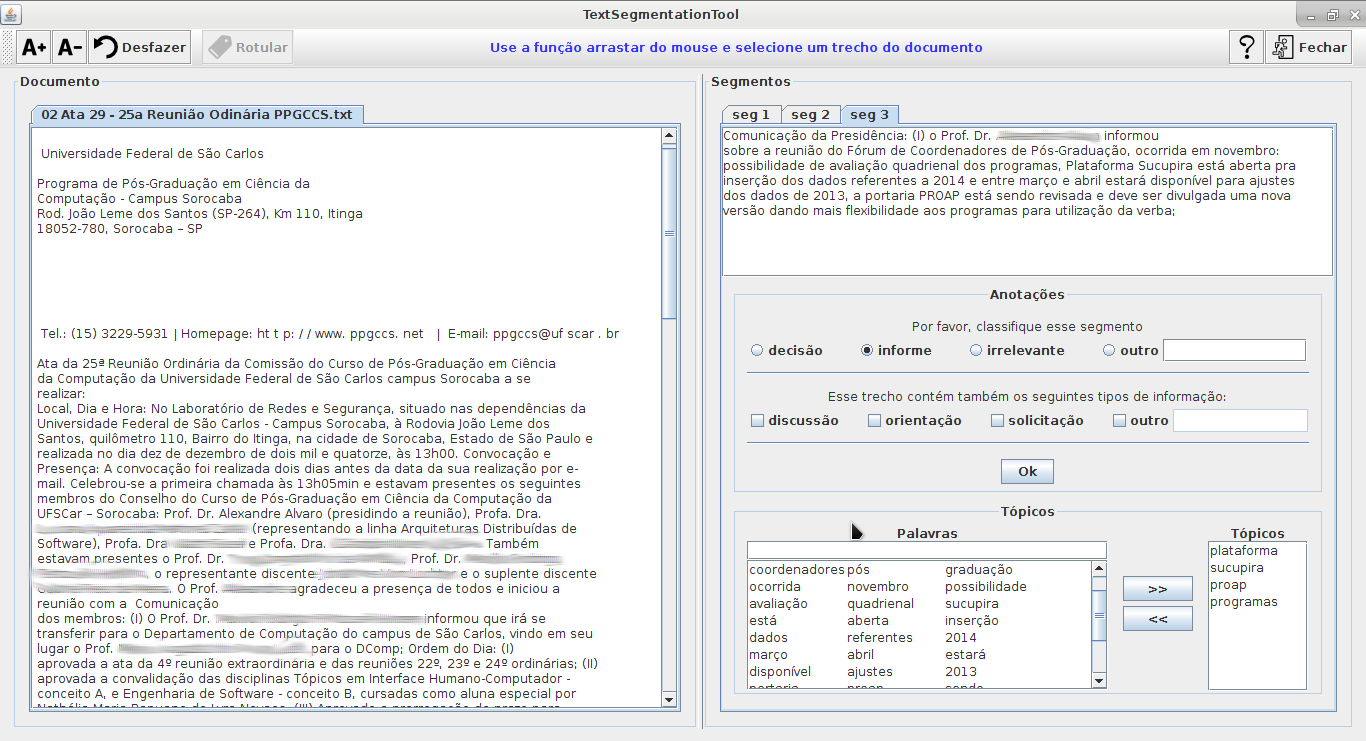
\includegraphics[width=\textwidth]{images/interface-TST.png}
\end{frame}


\begin{frame}{Descrição dos resultados obtidos com anotadores}
	\center Descrição dos resultados obtidos com anotadores
\tiny
\begin{table}[!h]
	\centering


	\begin{tabular}{|l|c|c|c|c|c|c|c|c|c|c|c|c|c|} \hline
		\textbf{Ata} & \textbf{\#Sent.}  & \textbf{A1}  & \textbf{A2}  & \textbf{A3}  & \textbf{A4}  & \textbf{A5}  & \textbf{A6}  & \textbf{A7}  & \textbf{A8}  & \textbf{A9} \\	\hline
% 		              A1   A2   A3  A4    A5   A6   A7   A8   A9   
		Ata 1  & 25 & 7  & 4  & 11 & 6  & 16 & 8  & 8  & 15 & 16 \\ \hline 
		Ata 2  & 17 & 4  & 4  & 8  & 6  & 11 & 6  & 6  & 15 & 14 \\ \hline 
		Ata 3  & 26 & 6  & 6  & 8  & 4  & 15 & 9  & 10 & 18 & 14 \\ \hline 
		Ata 4  & 26 & 5  & 5  & 10 & 6  & 14 & 17 & 7  & 11 & 12 \\ \hline 
		Ata 5  & 33 & 4  & 4  & 6  & 5  & 17 & 22 & 9  & 18 & 16 \\ \hline 
		Ata 6  & 11 & 3  & 4  & 6  & 4  & 9  & 9  & 4  & 7  &  5 \\ \hline 
		Ata 7  & 20 & 3  & 7  & 5  & 4  & 11 & 14 & 5  & 5  &  4 \\ \hline 
		Ata 8  & 35 & 4  & 8  & 3  & 8  & 12 & 17 & 5  & 11 &  9 \\ \hline 
		Ata 9  & 24 & 3  & 5  & 3  & 6  & 11 & 11 & 3  & 9  &  9 \\ \hline 
		Ata 10 & 50 & 4  & 5  & 4  & 7  & 31 & 29 & 5  & 9  &  8 \\ \hline 
		Ata 11 & 43 & 4  & 7  & 5  & 7  & 29 & 19 & 5  & 9  & 12 \\ \hline 
		Ata 12 & 56 & 3  & 10 & 4  & 16 & 33 & 25 & 4  & 13 & 11 \\ \hline 
		\textbf{Total} & \textbf{366} & \textbf{50}&  \textbf{69} & \textbf{73}&  \textbf{79}&  \textbf{209} & \textbf{186}&  \textbf{71}&  \textbf{140}&  \textbf{130} \\ \hline 

	\end{tabular}
	% \caption{Descrição dos resultados obtidos com anotadores. Na segunda coluna \#Sent., é mostrada a quantidade de sentenças de cada ata. Nas colunas A1-A9 é mostrado as quantidades de segmentos informados pelos anotadores. 
	% As colunas K, P$_k$ e WD indicam respectivamente as médias de \textit{Kappa}, $P_k$ e \textit{WindowDiff}.
% } 

\end{table}


\end{frame}








\begin{frame}{Exemplo de criação de uma segmentação de referência}


  \begin{center}
	  Referência criada a partir da concordância entre segmentações manuais.
	\begin{figure}[h!]

	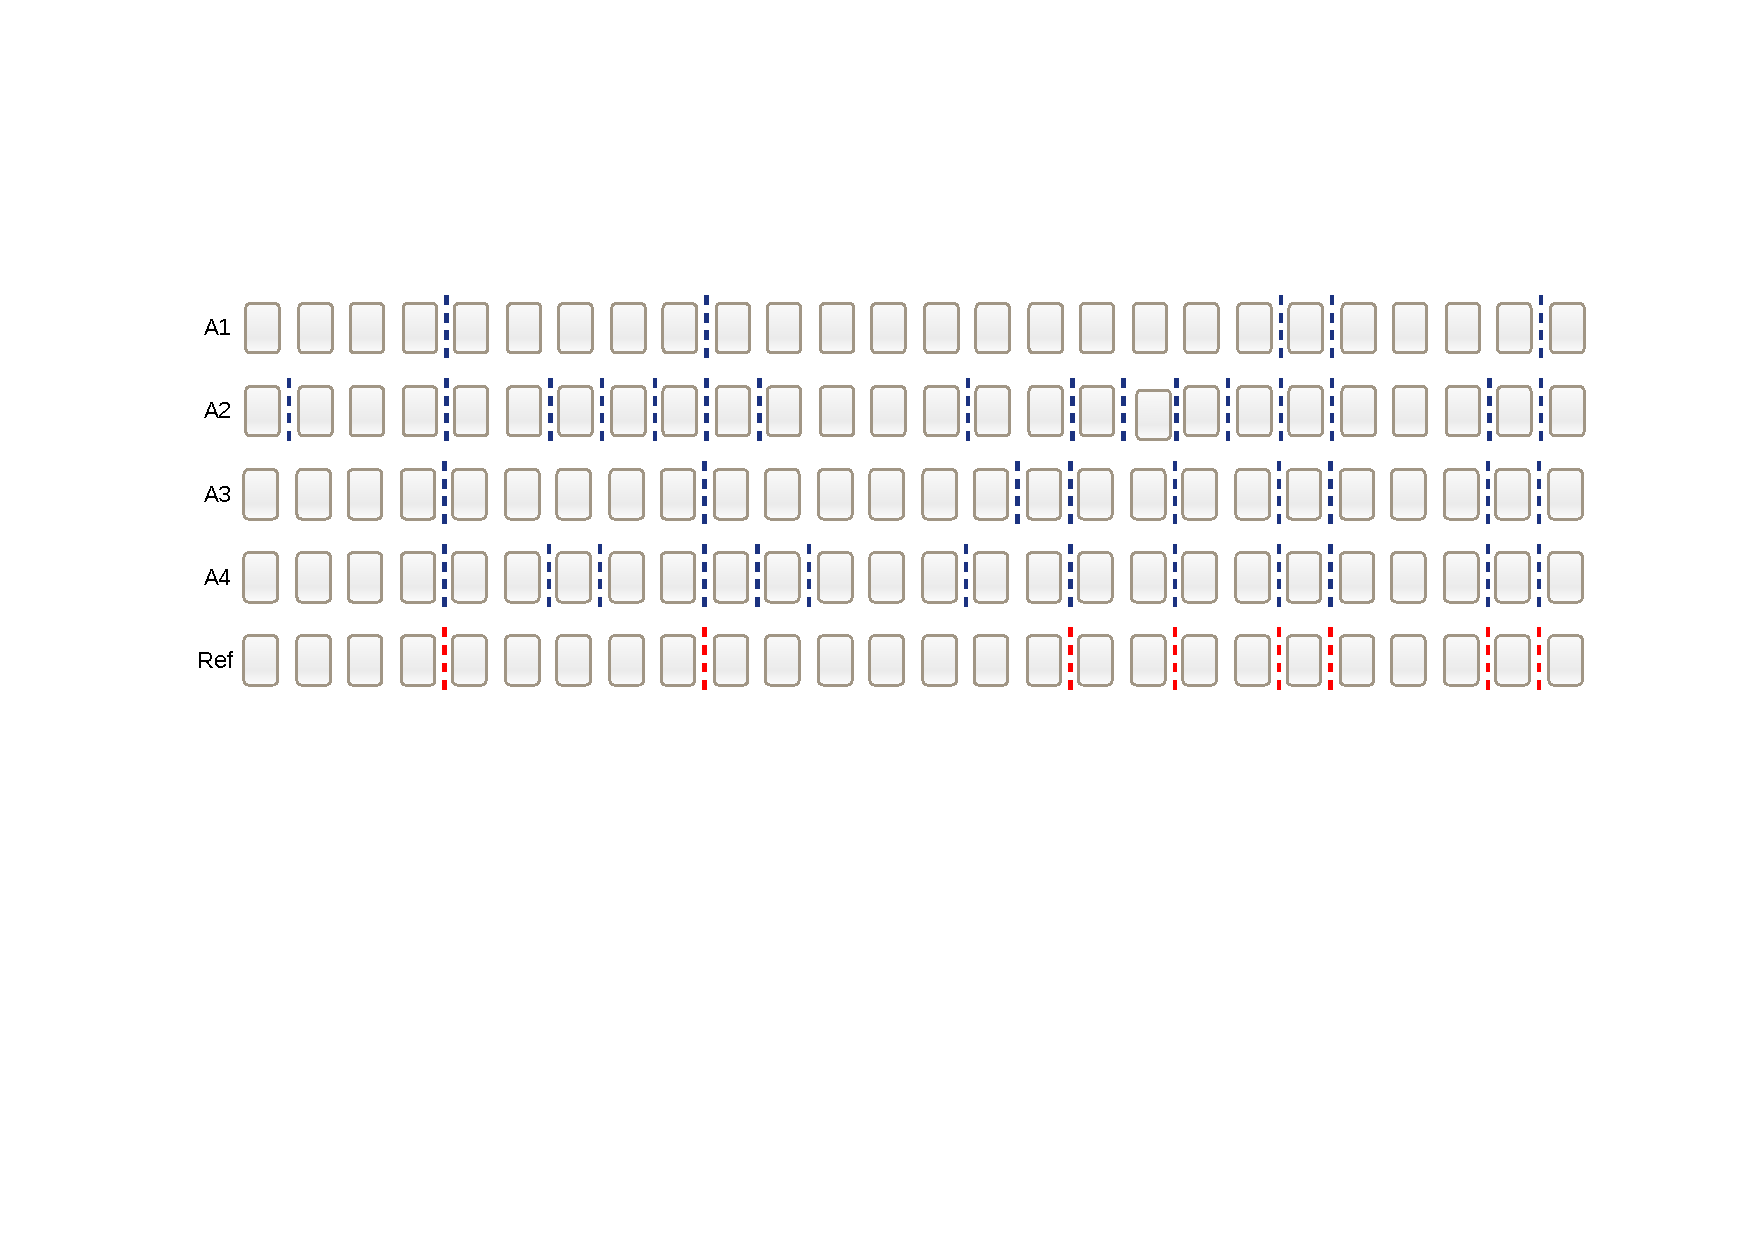
\includegraphics[trim={ 95 255 75 140 },clip,page=1,width=1\textwidth]{images/segmentacao-referencia.pdf}

	% \caption{Exemplo uma segmentação de referência criada a partir da concordância entre segmentações manuais.}
	\end{figure}


\end{center}


\end{frame}


% \begin{frame}{Segmentações de Referência}


	% \nblock{}{
		% Gerou-se 12 referências
		% \begin{itemize}
			% \item Segmentação;
			% \item Rótulos;
			% \item Descrição.
		% \end{itemize}
	% }


% \end{frame}





\begin{frame}{Configuração Experimental - Segmentadores}
\small

\begin{table}
\begin{tabular}{l|llllll}
	\textbf{Algoritmo} & \multicolumn{3}{l}{\textbf{Parâmetros} (Configuração)} \\
	% Algoritmo & P & \\
% \multicolumn{2}{c}{Multi-column}
\hline \hline
% (Configuração)

\textit{TextTiling} & \textbf{Win} &(20-60)  & \textbf{Step}   &(30-55)                  \\ 
\textit{C99} &        \textbf{SR} &(.2-.7)       & \textbf{W}      &(sim/não) & \textbf{RS}   &(3-7)        \\ 
\textit{BayesSeg} &   \textbf{SR} &(auto, .3-.9) & \textbf{Prior}  &(.08-.11) & \textbf{Disp} &(.1-.7)         \\ 
\textit{MinCut} &     \textbf{SR} &(.2-.7)       & \textbf{LenCut} &(5-15)                             \\ 
\textit{TextSeg} &    \textbf{SR} &(auto, .1-.9) &&&                                      \\ 
\textit{PseudoSeg} &  && &&&      \\ 

\end{tabular}
\end{table}


\end{frame}




\begin{frame}{Configuração Experimental}

% --------------------------------------------------

	\center Resumo dos melhores resultados obtidos por cada configuração


\begin{table}[!h]
	\centering
	\begin{tabular}{|l||c|c|c|c|c|c|c|c|c|c|c|} \hline

		\textbf{Algoritmo} && 
		\textbf{Step} &
		\textbf{Win} & 
		\textbf{P$_k$} & 
		\textbf{WD} & 
		\textbf{Ac} & 
		\textbf{Pr} & 
		\textbf{Re} &
		\textbf{F$^1$} &
		\textbf{\#Segs} \\	\hline

TextTiling && 20 & 30 & 0.461 & 0.444 & 0.581 & 0.560 & \cellcolor{gray!20} \textbf{0.336} & \cellcolor{gray!20} \textbf{0.411} & 8.833  \\ \hline 
TextTiling && 30 & 45 & \cellcolor{gray!20} \textbf{0.450} & \cellcolor{gray!20} \textbf{0.435} & \cellcolor{gray!20} \textbf{0.596} & \cellcolor{gray!20} \textbf{0.696} & 0.275 & 0.373 & 6.417  \\ \hline 

\hline
		\textbf{Algoritmo} &
		\textbf{RS} &
		\textbf{W} & 
		\textbf{SRate}& 
		\textbf{P$_k$} & 
		\textbf{WD} & 
		\textbf{Ac} & 
		\textbf{Pr} & 
		\textbf{Re} &
		\textbf{F$^1$} &
		\textbf{\#Segs} \\	\hline

C99 & 3 & true  &0.300 &  \cellcolor{gray!20} \textbf{0.434} & \cellcolor{gray!20} \textbf{0.407} & 0.607 & 0.655 & 0.376 & 0.457 & 9.250  \\ \hline 
C99 & 3 & true  &0.700 &  0.485 & 0.431 & 0.602 & 0.553 & \cellcolor{gray!20} \textbf{0.797} & \cellcolor{gray!20} \textbf{0.633} & 21.417  \\ \hline 
C99 & 5 & true  &0.500 &  0.460 & 0.421 & \cellcolor{gray!20} \textbf{0.609} & 0.580 & 0.600 & 0.571 & 15.500  \\ \hline 
C99 & 3 & false &0.200 &  0.448 & 0.427 & 0.596 & \cellcolor{gray!20} \textbf{0.719} & 0.257 & 0.362 & 6.083  \\ \hline 


\hline
		\textbf{Algoritmo} && 
		\textbf{Cut} & 
		\textbf{SRate} &
		\textbf{P$_k$} & 
		\textbf{WD} & 
		\textbf{Ac} & 
		\textbf{Pr} & 
		\textbf{Re} &
		\textbf{F$^1$} &
		\textbf{\#Segs} \\	\hline


MinCutSeg && 13 & 0.300 & 0.457 & 0.427 & 0.594 & \cellcolor{gray!20} \textbf{0.638} & 0.353 & 0.433 & 8.667  \\ \hline 
MinCutSeg && 9  & 0.400 & \cellcolor{gray!20} \textbf{0.444} & 0.408 & \cellcolor{gray!20} \textbf{0.614} & 0.629 & 0.494 & 0.526 & 11.917  \\ \hline 
MinCutSeg && 11 & 0.500 & 0.459 & \cellcolor{gray!20} \textbf{0.407} & 0.603 & 0.588 & 0.590 & 0.563 & 15.000  \\ \hline 
MinCutSeg && 5  & 0.700 & 0.528 & 0.438 & 0.567 & 0.536 & \cellcolor{gray!20} \textbf{0.746} & \cellcolor{gray!20} \textbf{0.599} & 21.000  \\ \hline 


\hline
		\textbf{Algoritmo} &
		\textbf{Prior} &
		\textbf{Disp.} & 
		\textbf{SRate}& 
		\textbf{P$_k$} & 
		\textbf{WD} & 
		\textbf{Ac} & 
		\textbf{Pr} & 
		\textbf{Re} &
		\textbf{F$^1$} &
		\textbf{\#Segs} \\	\hline


 BayesSeg & 0.0800 & 0.5000 &  Auto & \cellcolor{gray!20} \textbf{0.380} & \cellcolor{gray!20} \textbf{0.361} & \cellcolor{gray!20} \textbf{0.655} & 0.662 & 0.479 & 0.551 & 10.000  \\ \hline 
 BayesSeg & 0.1100 & 0.5000 &  Auto & 0.388 & 0.370 & 0.649 & \cellcolor{gray!20} \textbf{0.672} & 0.433 & 0.523 & 9.000  \\ \hline 
 BayesSeg & 0.1100 & 0.1000 & 0.600 & 0.462 & 0.399 & 0.615 & 0.574 & 0.724 & \cellcolor{gray!20} \textbf{0.619} & 18.417  \\ \hline 
 BayesSeg & 0.0800 & 0.1000 & 0.900 & 0.645 & 0.517 & 0.490 & 0.478 & \cellcolor{gray!20} \textbf{0.878} & 0.600 & 27.500  \\ \hline 

\hline
		\textbf{Algoritmo} &&&
		\textbf{SRate} & 
		\textbf{P$_k$} & 
		\textbf{WD} & 
		\textbf{Ac} & 
		\textbf{Pr} & 
		\textbf{Re} &
		\textbf{F$^1$} &
		\textbf{\#Segs} \\	\hline

TextSeg &&& Auto & \cellcolor{gray!20} \textbf{0.455} & 0.439 & 0.585 & \cellcolor{gray!20} \textbf{0.618} & 0.266 & 0.368 & 6.417  \\ \hline 
TextSeg &&& 0.500 & 0.475 & \cellcolor{gray!20} \textbf{0.417} & \cellcolor{gray!20} \textbf{0.594} & 0.565 & 0.608 & 0.566 & 15.500  \\ \hline 
TextSeg &&& 0.900 & 0.604 & 0.484 & 0.524 & 0.498 & \cellcolor{gray!20} \textbf{0.922} & \cellcolor{gray!20} \textbf{0.627} & 27.500  \\ \hline 

\hline
		\textbf{Algoritmo} &&&
		\textbf{SRate} & 
		\textbf{P$_k$} & 
		\textbf{WD} & 
		\textbf{Ac} & 
		\textbf{Pr} & 
		\textbf{Re} &
		\textbf{F$^1$} &
		\textbf{\#Segs} \\	\hline


Sentenças &&& 1.000& \cellcolor{gray!20} \textbf{0.640} & \cellcolor{gray!20} \textbf{0.490} & \cellcolor{gray!20} \textbf{0.506} & \cellcolor{gray!20} \textbf{0.488} & \cellcolor{gray!20} \textbf{1.000} & \cellcolor{gray!20} \textbf{0.638} & 30.500  \\ \hline 



	\end{tabular}
	\caption{Resultados}
	\label{tab:resumo-resultados}
\end{table}


 

% -------------------------------------------------- 

\end{frame}









\begin{frame}{Avaliação Experimental}

	\center Influência da taxa de segmentos na eficiência dos algoritmos

\begin{figure}[!h] \centering     %%% not \center
	  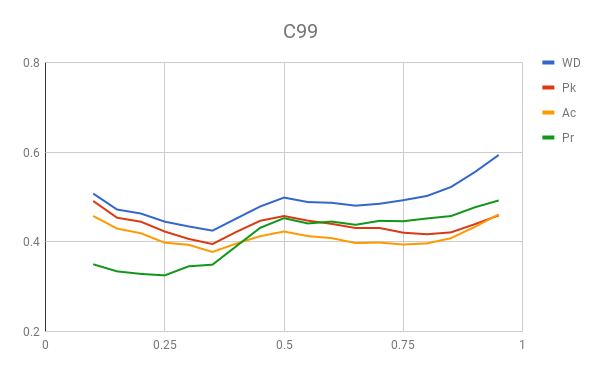
\includegraphics[width=.48\textwidth]{images/graficos/analiseNSegRate-C99.png}
	  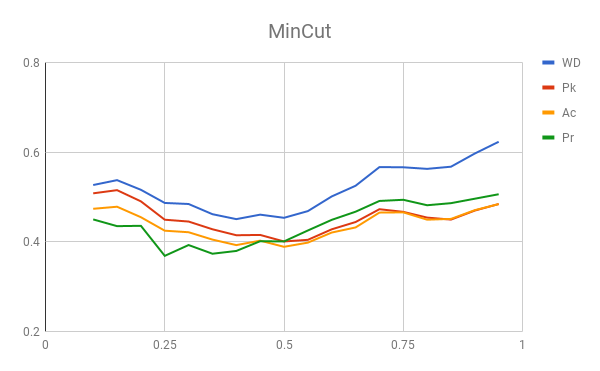
\includegraphics[width=.48\textwidth]{images/graficos/analiseNSegRate-MinCut.png} \\
	  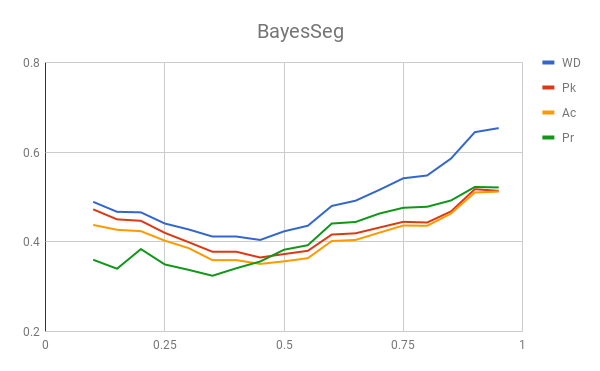
\includegraphics[width=.48\textwidth]{images/graficos/analiseNSegRate-Bayes.png}
	  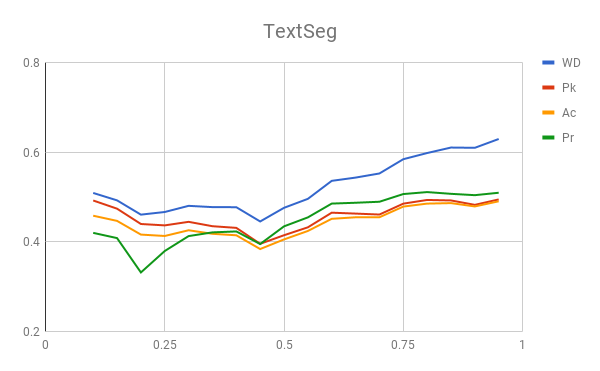
\includegraphics[width=.48\textwidth]{images/graficos/analiseNSegRate-UISeg.png}
\end{figure}


\end{frame}







\begin{frame}{Avaliação Experimental}



\eblock{}{
	Testes de significância estatística de Friedman com pós teste de Nemenyi

	\begin{itemize}
		\item Inicialmente com as configurações de cada algoritmo.
			% cada algoritmo para encontrar a melhor configuração.
		\item Novamente com as melhores configurações de cada algoritmo.
	\end{itemize}
}



\end{frame}








\begin{frame}{Avaliação Experimental}

\small\center Diagramas de Diferença Crítica sobre \textit{ranking} considerando valores de Acurácia, $F^1$, \textit{WindowDiff}, e $P_k$.

\begin{figure}[!h]
	\centering     %%% not \center
\tiny
	\subfigure[Ac]{ \label{fig:a}
		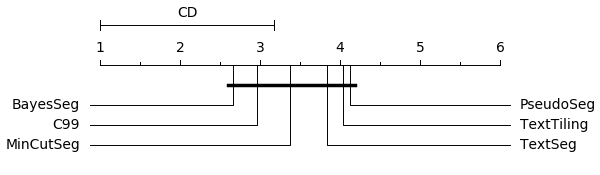
\includegraphics[width=47mm]{images/cds/Acuracia.png} 
	}	
	\subfigure[F^1]{ \label{fig:b}
		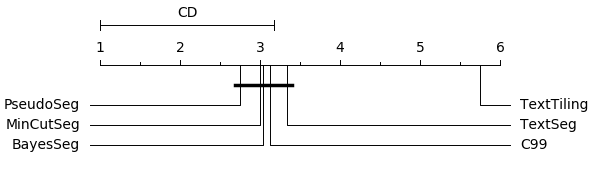
\includegraphics[width=47mm]{images/cds/F1.png} \\
	}
	\subfigure[P_k]{ \label{fig:c}
		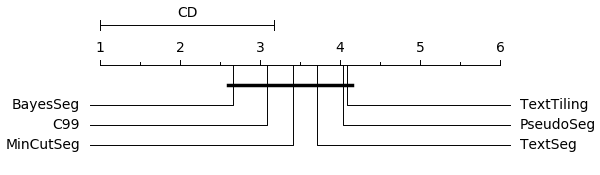
\includegraphics[width=47mm]{images/cds/Pk.png} 
	}
	\subfigure[WD]{ \label{fig:d}
		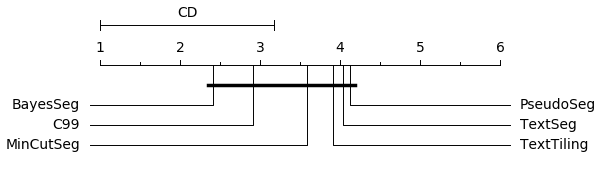
\includegraphics[width=47mm]{images/cds/WD.png} 
	}

		% \caption{
% }
	% \label{fig:CDs}

	
\end{figure}
Não há diferença significativa entre os métodos.
	
\end{frame}
	










\begin{frame}{Avaliação Experimental}

Os modelos de Extração de Tópicos foram avaliados junto aos usuários.



\nblock{}{
\begin{itemize}
	\item Resultados de 2 consultas ao Sistema usando 
	\item 3 Extratores (K-Means, LDA, PLSA);
	\item Impressões dos usuários coletadas via questionários.
\end{itemize}
}

\end{frame}




\begin{frame}{Consultas ao Sistema}


\nblock{}{
	Entrada:
\begin{enumerate}
	\item \textit{``defesa de dissertação''};
	\item \textit{``compra de equipamentos''}.
\end{enumerate}
}

\nblock{}{
	\textit{Corpus} 
	\begin{itemize}
		\item Formado por 175 atas; 
		\item Segmentadas com o \textit{BayesSeg};
		\item Conjunto de 1276 segmentos. 
	\end{itemize}
}

\nblock{}{
	Resultados utilizando 3 modelos para Extração de Tópicos:
\begin{enumerate}
	\item K-Means;
	\item LDA;
	\item PLSA.
\end{enumerate}
}


\end{frame}


\begin{frame}{Avaliação Subjetiva}

	\nblock{}{
		Os resultados foram apresentados à um grupo de avaliadores:

		\begin{itemize}
			\item 24 profissionais da UFSCar;
			\item 13 profissionais de escolas técnicas;
			\item 03 profissionais de escolas do Ensino Fundamental.
		\end{itemize}
	}

	\nblock{}{
		Perfil:
		\begin{itemize}
			\item 17 membros de conselhos;
			\item 12 gestores;
			\item 05 administrativos;
			\item 03 professores;
			\item 03 sem afinidade com atas (descartados).
		\end{itemize}
	}

\end{frame}




\begin{frame}{Questionário}
	\nblock{}{
		Coletar respostas referentes à:
		\begin{enumerate}
			\item Coesão dos tópicos;
			\item Representatividade dos descritores;
			\item Coesão dos segmentos;
			\item Completude dos segmentos.
		\end{enumerate}
	}
	
\end{frame}




\begin{frame}{Coesão dos tópicos}

	\center \small 
	Primeira questão:\textit{``Todos os trechos apresentados compartilham um mesmo assunto.''}. 

\begin{figure}[!h] \centering     %%% not \center
		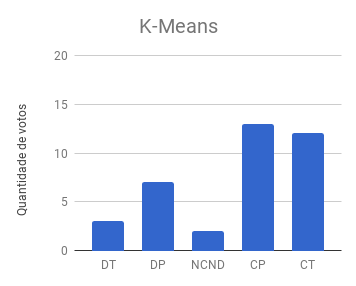
\includegraphics[width=.31\textwidth]{images/figuras-experimento/Q1-KMeans.png}
		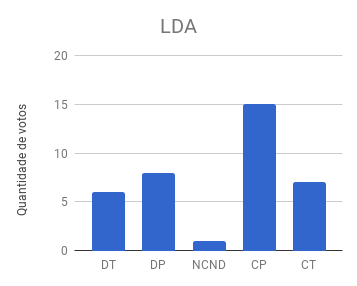
\includegraphics[width=.31\textwidth]{images/figuras-experimento/Q1-LDA.png}
		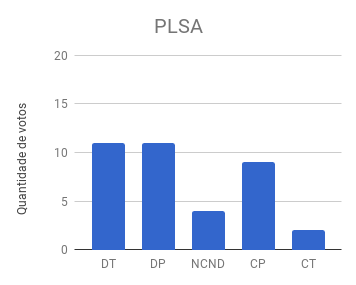
\includegraphics[width=.31\textwidth]{images/figuras-experimento/Q1-PLSA.png}
	\label{fig:Q1}
\end{figure}


\begin{figure}[!h] \centering     %%% not \center
	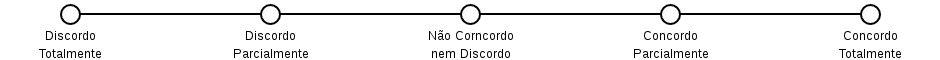
\includegraphics[width=.9\textwidth]{images/likert.png}
\end{figure}


\end{frame}



\begin{frame}{Representatividade dos descritores}

	\center\small 
	Segunda questão:\textit{``As palavras \textit{$<$descritores$>$} resumem bem o assunto tratado nos trechos.''}.

\begin{figure}[!h] \centering     %%% not \center

	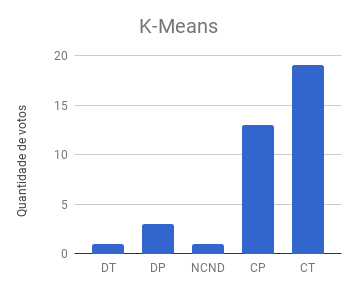
\includegraphics[width=.31\textwidth]{images/figuras-experimento/Q2-KMeans.png}
	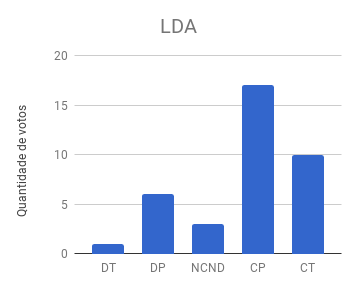
\includegraphics[width=.31\textwidth]{images/figuras-experimento/Q2-LDA.png}
	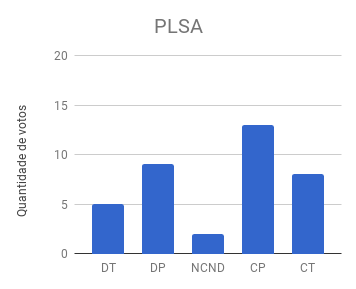
\includegraphics[width=.31\textwidth]{images/figuras-experimento/Q2-PLSA.png}
\end{figure}

\begin{figure}[!h] \centering     %%% not \center
	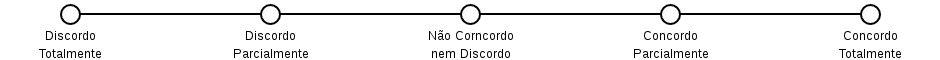
\includegraphics[width=.9\textwidth]{images/likert.png}
\end{figure}

\end{frame}



\begin{frame}{Coesão dos segmentos}

	\center \small 
	Terceira questão:\textit{``Existem trechos que não tratam de um único assunto?''}. 

\begin{figure}[!h] \centering     %%% not \center
	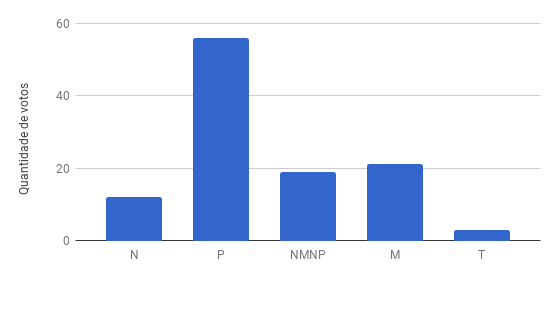
\includegraphics[width=.48\textwidth]{images/figuras-experimento/Q3-Seg.png}
\end{figure}


\begin{figure}[!h] \centering     %%% not \center
	
\includegraphics[width=.9\textwidth]{images/likert-1.png}
\end{figure}


\end{frame}



\begin{frame}{Completude dos Segmentos}

	\center \small 
	Quarta questão:\textit{``Existem trechos incompletos e insuficientes para compreensão do assunto do trecho?''}.


\begin{figure}[!h] \centering     %%% not \center

	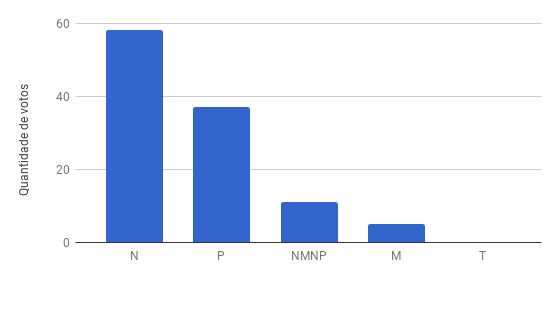
\includegraphics[width=.48\textwidth]{images/figuras-experimento/Q4-Seg.png}
	\label{fig:Q4}
\end{figure}

\begin{figure}[!h] \centering     %%% not \center
	
\includegraphics[width=.9\textwidth]{images/likert-1.png}
\end{figure}

\end{frame}




\begin{frame}{Comportamento em consultas diferentes}

	\center 
	Coesão dos tópicos\\
	\tiny Primeira questão:\textit{``Todos os trechos apresentados compartilham um mesmo assunto.''}. 

\begin{figure}[!h] \centering     %%% not \center

		\tiny Primeira Consulta: \textit{``defesa de dissertação''}
		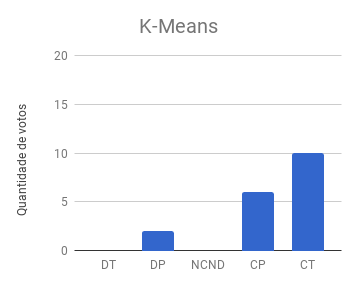
\includegraphics[width=.31\textwidth]{images/figuras-experimento/C1-Q1-KMeans.png}
		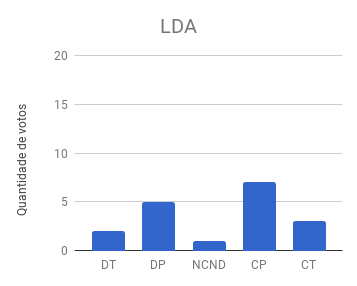
\includegraphics[width=.31\textwidth]{images/figuras-experimento/C1-Q1-LDA.png}
		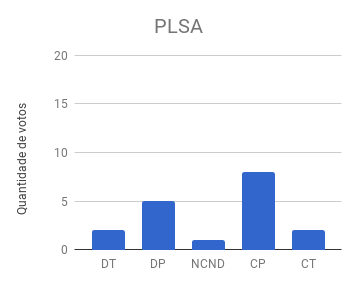
\includegraphics[width=.31\textwidth]{images/figuras-experimento/C1-Q1-PLSA.png} 
		\\
		% \vspace{1cm}
		Segunda Consulta: \textit{``compra de equipamentos''}
		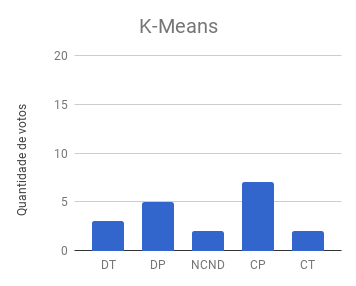
\includegraphics[width=.31\textwidth]{images/figuras-experimento/C2-Q1-KMeans.png}
		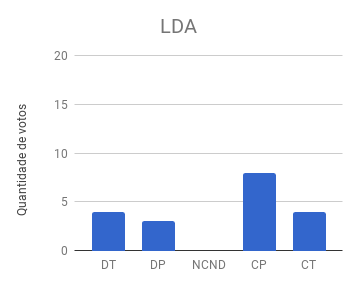
\includegraphics[width=.31\textwidth]{images/figuras-experimento/C2-Q1-LDA.png}
		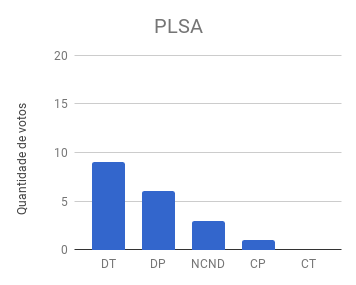
\includegraphics[width=.31\textwidth]{images/figuras-experimento/C2-Q1-PLSA.png}

	% \caption{Contagem das respostas referentes a Primeira questão. A primeira consulta, ``\textit{compra de equipamentos}'', é mostrada na linha superior e a segunda consulta, ``\textit{defesa de dissertação}'', na linha inferior.}
	

\end{figure}


\end{frame}





\begin{frame}{Comportamento dos extratores em consultas diferentes}

	\center 
	Representatividade dos descritores\\
	\tiny Segunda questão:\textit{``As palavras \textit{$<$descritores$>$} resumem bem o assunto tratado nos trechos.''}.

\begin{figure}[!h] \centering     %%% not \center

		\tiny Primeira Consulta: \textit{``defesa de dissertação''}
		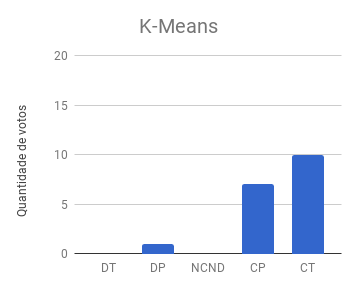
\includegraphics[width=.31\textwidth]{images/figuras-experimento/C1-Q2-KMeans.png}
		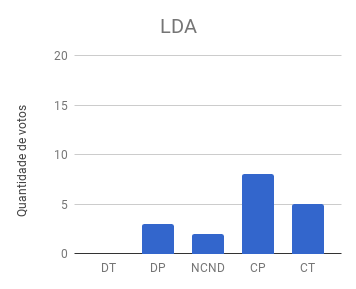
\includegraphics[width=.31\textwidth]{images/figuras-experimento/C1-Q2-LDA.png}
		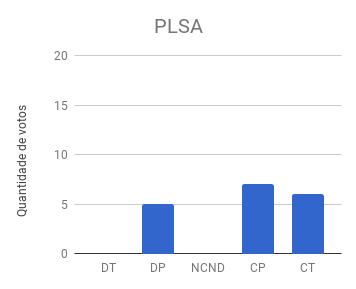
\includegraphics[width=.31\textwidth]{images/figuras-experimento/C1-Q2-PLSA.png}
		\\
		% \vspace{1cm}
		Segunda Consulta: \textit{``compra de equipamentos''}
		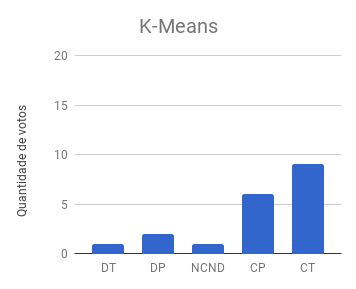
\includegraphics[width=.31\textwidth]{images/figuras-experimento/C2-Q2-KMeans.png}
		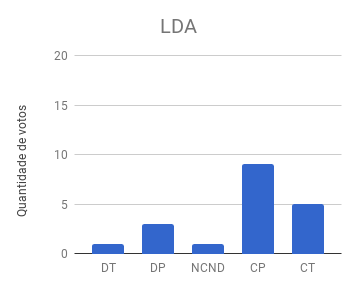
\includegraphics[width=.31\textwidth]{images/figuras-experimento/C2-Q2-LDA.png}
		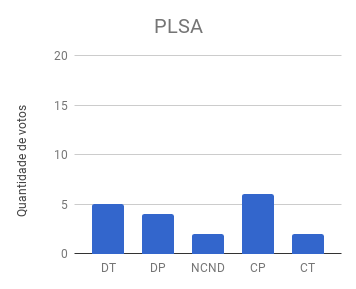
\includegraphics[width=.31\textwidth]{images/figuras-experimento/C2-Q2-PLSA.png}

		% \caption{Contagem das respostas referentes a Segunda questão. A primeira consulta, ``\textit{compra de equipamentos}'', é mostrada na linha superior e a segunda consulta, ``\textit{defesa de dissertação}'', na linha inferior.}


\end{figure}

\end{frame}





\begin{frame}{Qualidade dos segmentos apresentados em diferentes técnicas}

\center Coesão dos segmentos\\
\tiny Terceira questão:\textit{``Existem trechos que não tratam de um único assunto?''}.%  
	\vspace{1cm}

\begin{figure}[!h] \centering     %%% not \center

		\includegraphics[width=.31\textwidth]{images/figuras-experimento/t1q3.png}
		\includegraphics[width=.31\textwidth]{images/figuras-experimento/t2q3.png}
		\includegraphics[width=.31\textwidth]{images/figuras-experimento/t3q3.png}

	% \caption{Contagem das respostas referentes a terceira questão, isolando-se as técnicas de extração de tópicos.}

\end{figure}



\end{frame}




\begin{frame}{Qualidade dos segmentos apresentados em diferentes técnicas}

\center Completude dos Segmentos\\
\tiny Quarta questão:\textit{``Existem trechos incompletos e insuficientes para compreensão do assunto do trecho?''}.%
	\vspace{1cm}

\begin{figure}[!h] \centering     %%% not \center

		\includegraphics[width=.31\textwidth]{images/figuras-experimento/t1q4.png}
		\includegraphics[width=.31\textwidth]{images/figuras-experimento/t2q4.png}
		\includegraphics[width=.31\textwidth]{images/figuras-experimento/t3q4.png}

	% \caption{Contagem das respostas referentes a quarta questão, isolando-se as técnicas de extração de tópicos.}
	\label{fig:influenciaExtSegQ4}
\end{figure}

\end{frame}






















% ---------- Conclusão ----------
\section{Conclusão}
\begin{frame}{Conclusão}
	
\nblock{}{
	A metodologia utilizada nesse trabalho: 
\begin{itemize}
	\item Conecta as técnicas de segmentação textual aos modelos de Extração de Tópicos; 
	\item Gera um estrutura derivada de um \textit{corpus} não estruturado;
	% \item Descobre e identifica variáveis latentes pa
	\item Utiliza variáveis latentes em conjunto com técnicas de Recuperação de Informação.
\end{itemize}
}
\end{frame}




\begin{frame}{Conclusão}
	\center Segmentação 

	\nblock{}{
		Resultados:
	\begin{itemize}
		\item Medidas abaixo do esperado;
		\item Impressões satisfatórias dos usuários;
			\begin{itemize}
				\item Completude;
				\item Coesão;
			\end{itemize}
	\end{itemize}
	}


	\nblock{}{
		Possíveis melhorias:
	\begin{itemize}
		\item Segmentação de referência com mais anotadores;
		\item Treinamento dos anotadores;
		\item Maior concordância entre anotadores;
		\item Segmentação de referência mais confiável e representativa.
	\end{itemize}
	}

\end{frame}





\begin{frame}{Conclusão}

	\center Extração de Tópicos
	\nblock{}{
	\begin{itemize}
		\item Extraem padrões úteis do \textit{corpus};
		\item Melhores resultados com o K-Means;
			\begin{itemize}
				\item Coesão dos grupos;
				\item Capacidade Representativa do descritores;
			\end{itemize}
			% \begin{itemize}
				% \item Coesão 
				% \item Representatividade
				% \item Discrepância entre as consultas;
			% \end{itemize}
	\end{itemize}
	}


	% \nblock{}{
	% \begin{itemize}
		% \item Discrepância entre as consultas;
	% \end{itemize}
	% }

\end{frame}



\begin{frame}{Conclusão}

	\nblock{} {
Contribuições:

	\begin{itemize}
\item O método para extração de conhecimento em documentos multi-temáticos; 
\item O corpus de atas anotadas;
\item A ferramenta para segmentação e anotação manual;
\item O Sistema proposto e sua implementação; 
\item As avaliações dos Segmentadores e Extratores de Tópicos.

	\end{itemize}
	}

	\eblock{} {
		\begin{itemize}
			\item Submissão de artigo.
		\end{itemize}
	}

\end{frame}










% ---------- Trabalhos Futuros ----------
\section{Trabalhos Futuros}
\begin{frame}{Trabalhos Futuros}
	
	\nblock{} {

		Conclusão do Sistema:
	\begin{itemize}
		\item Algoritmos de agrupamento incremental
		\item Classificação dos segmentos em relação ao tipo de menção ao assunto
	\end{itemize}
}
	
	\nblock{} {
		Melhorias:
	\begin{itemize}
		\item Inclusão de novos corpora (transcrições de conversas, diálogos em chats, discursos e atas de outras organizações)
		\item Fontes externas para melhorar os métodos de segmentação textual  (\textit{thesaurus} e \textit{clue words});
		\item Testes voltados a experiência do usuário.

	\end{itemize}
	
	}
\end{frame}



\begin{frame}{}

\center\LARGE Obrigado!

\end{frame}

\end{document}













%%%%%%%%%%%%%%%%%%%%%%%%%%%%%%%%%%%%%%%%%%%%%%%%%%%%%%%%%%
%%%%%%%%%%%%%%%%%%%%%%%%%%%%%%%%%%%%%%%%%%%%%%%%%%%%%%%%%%
%%%%%%%%%%%%%%% == FIM DA APRESENTAÇÃO == %%%%%%%%%%%%%%%%
%%%%%%%%%%%%%%%%%%%%%%%%%%%%%%%%%%%%%%%%%%%%%%%%%%%%%%%%%%
%%%%%%%%%%%%%%%%%%%%%%%%%%%%%%%%%%%%%%%%%%%%%%%%%%%%%%%%%%


\section{}
%%%%%%%%%%%%%%%%%%%%%%%%%%%%%%%%%%%%%%%%%%%%%%%%%%%%%%%%%%
\begin{frame}{}
	
	\nblock{}{
	
	}
	
\end{frame}
%%%%%%%%%%%%%%%%%%%%%%%%%%%%%%%%%%%%%%%%%%%%%%%%%%%%%%%%%%
	
